\chapter{Oporto WAN}

\section{Site Overview}

Oporto is the location of the headquarters of the \ac{RECOMP} Corporation and represents the most complex part of the \ac{WAN}. The site consists of the following devices:

\begin{itemize}
    \item One Router HQ (2911 model)
    \item Two Multilayer Switches MLS1 and MLS2 (3560-24PS model)
    \item Two Layer 2 switches (2960-24TT model)
    \item Four PCs representing each of the HQ networks: STAFF, ACCOUNTING, HR and USERS
\end{itemize}

The topology of the Oporto \ac{WAN} is illustrated in Figure~\ref{fig:opo-topology}, showing the connection between the router, multilayer switches, Layer 2 switches, and \ac{VLAN}s for each network.


\begin{figure}[!htb]
\centering
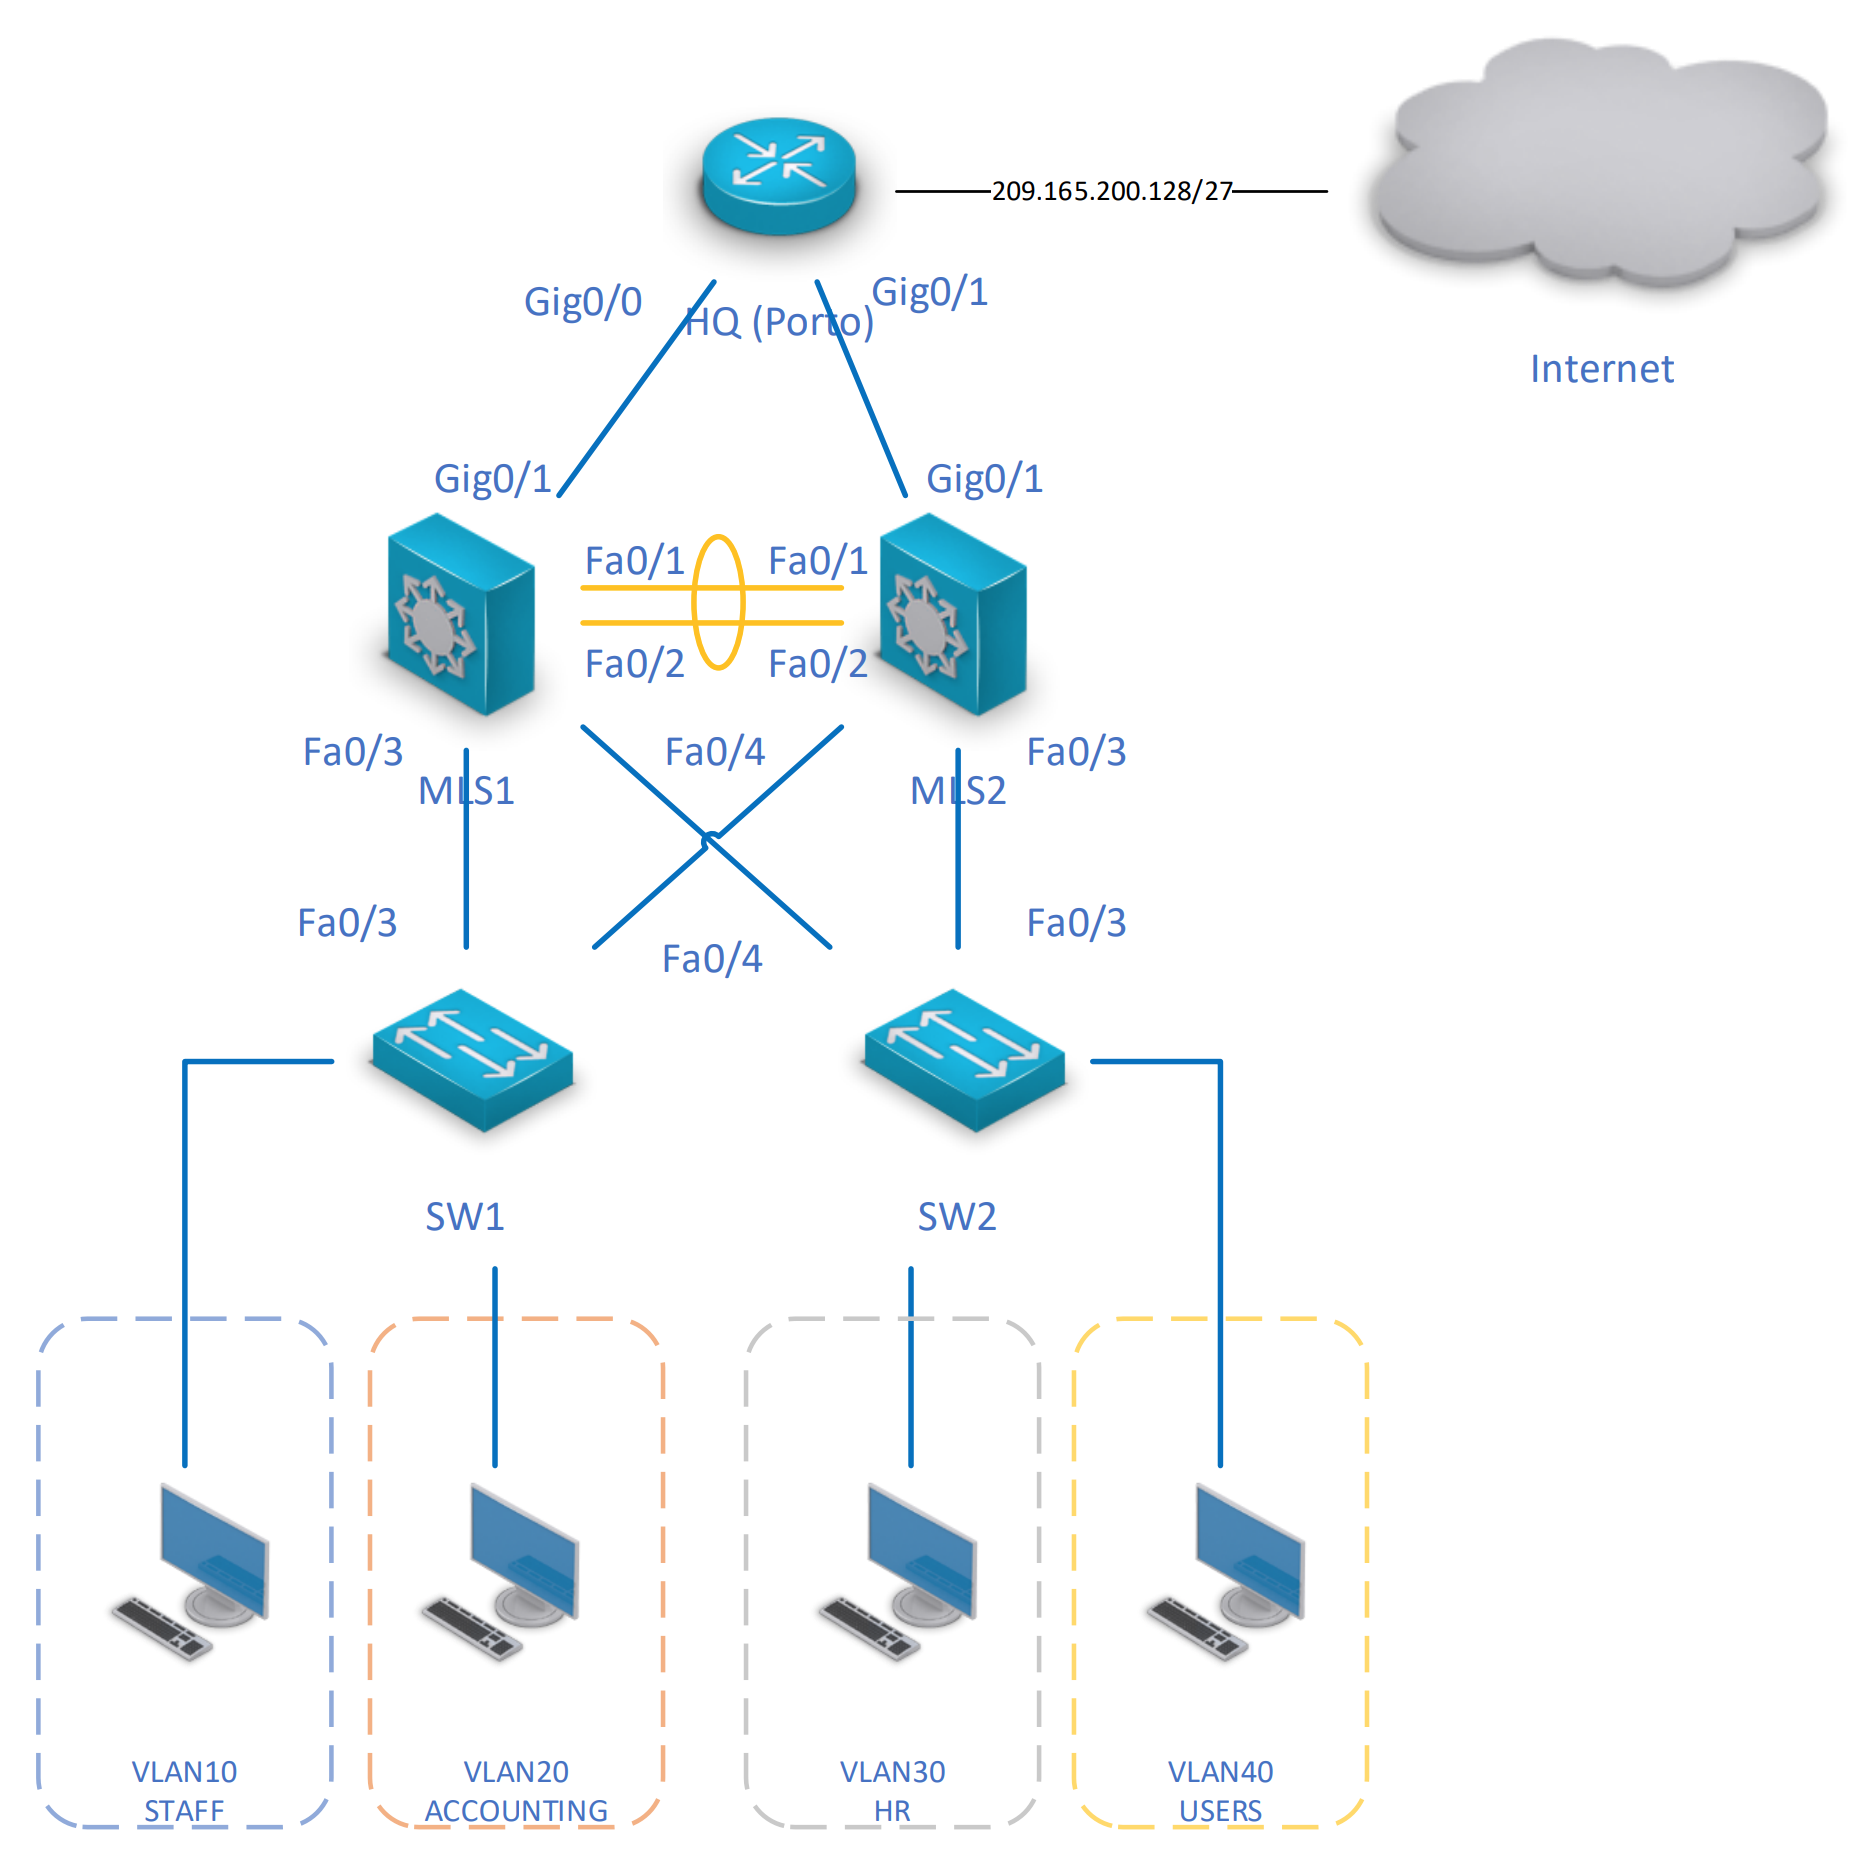
\includegraphics[width=0.5\textwidth]{figures/opo-topology.png}
\caption{Oporto WAN Topology\cite{recomp_sprint1}}
\label{fig:opo-topology}
\end{figure}


The \ac{VLAN}s assigned to the HQ networks are:

\begin{itemize}
    \item \ac{VLAN} 10: STAFF
    \item \ac{VLAN} 20: ACCOUNTING
    \item \ac{VLAN} 30: HR
    \item \ac{VLAN} 40: USERS
\end{itemize}

The Oporto \ac{WAN} is connected to the Internet using the address block 209.165.200.128/27.

\section{Oporto \ac{WAN} Addressing}

The \ac{IP} addressing scheme for the Oporto site was designed to accommodate the four internal networks while optimizing the available address space. The networks and their corresponding addresses are summarized in Table~\ref{tab:opo-addressing}.

\begin{table}[h]
\centering
\resizebox{\textwidth}{!}{%
\begin{tabular}{lccccc}
\hline
Network & Number of Nodes & Network Address & Broadcast Address & Mask & First--Last Valid Address \\
\hline
USERS & 500 & 10.21.44.0 & 10.21.45.255 & /23 & 10.21.44.1 -- 10.21.45.254 \\
ACCOUNTING & 200 & 10.21.46.0 & 10.21.46.255 & /24 & 10.21.46.1 -- 10.21.46.254 \\
HR & 100 & 10.21.47.0 & 10.21.47.127 & /25 & 10.21.47.1 -- 10.21.47.126 \\
STAFF & 50 & 10.21.47.128 & 10.21.47.191 & /26 & 10.21.47.129 -- 10.21.47.190 \\
HQ-ROUTER $\leftrightarrow$ MLS1 & 4 & 10.21.47.192 & 10.21.47.195 & /30 & 10.21.47.193-10.21.47.194 \\
HQ-ROUTER $\leftrightarrow$ MLS2 & 4 & 10.21.47.196 & 10.21.47.199 & /30 & 10.21.47.197-10.21.47.198 \\
\hline
\end{tabular}%
}
\caption{Oporto \ac{WAN} \ac{IP} addressing scheme.}
\label{tab:opo-addressing}
\end{table}


\begin{figure}[!htb]
\centering
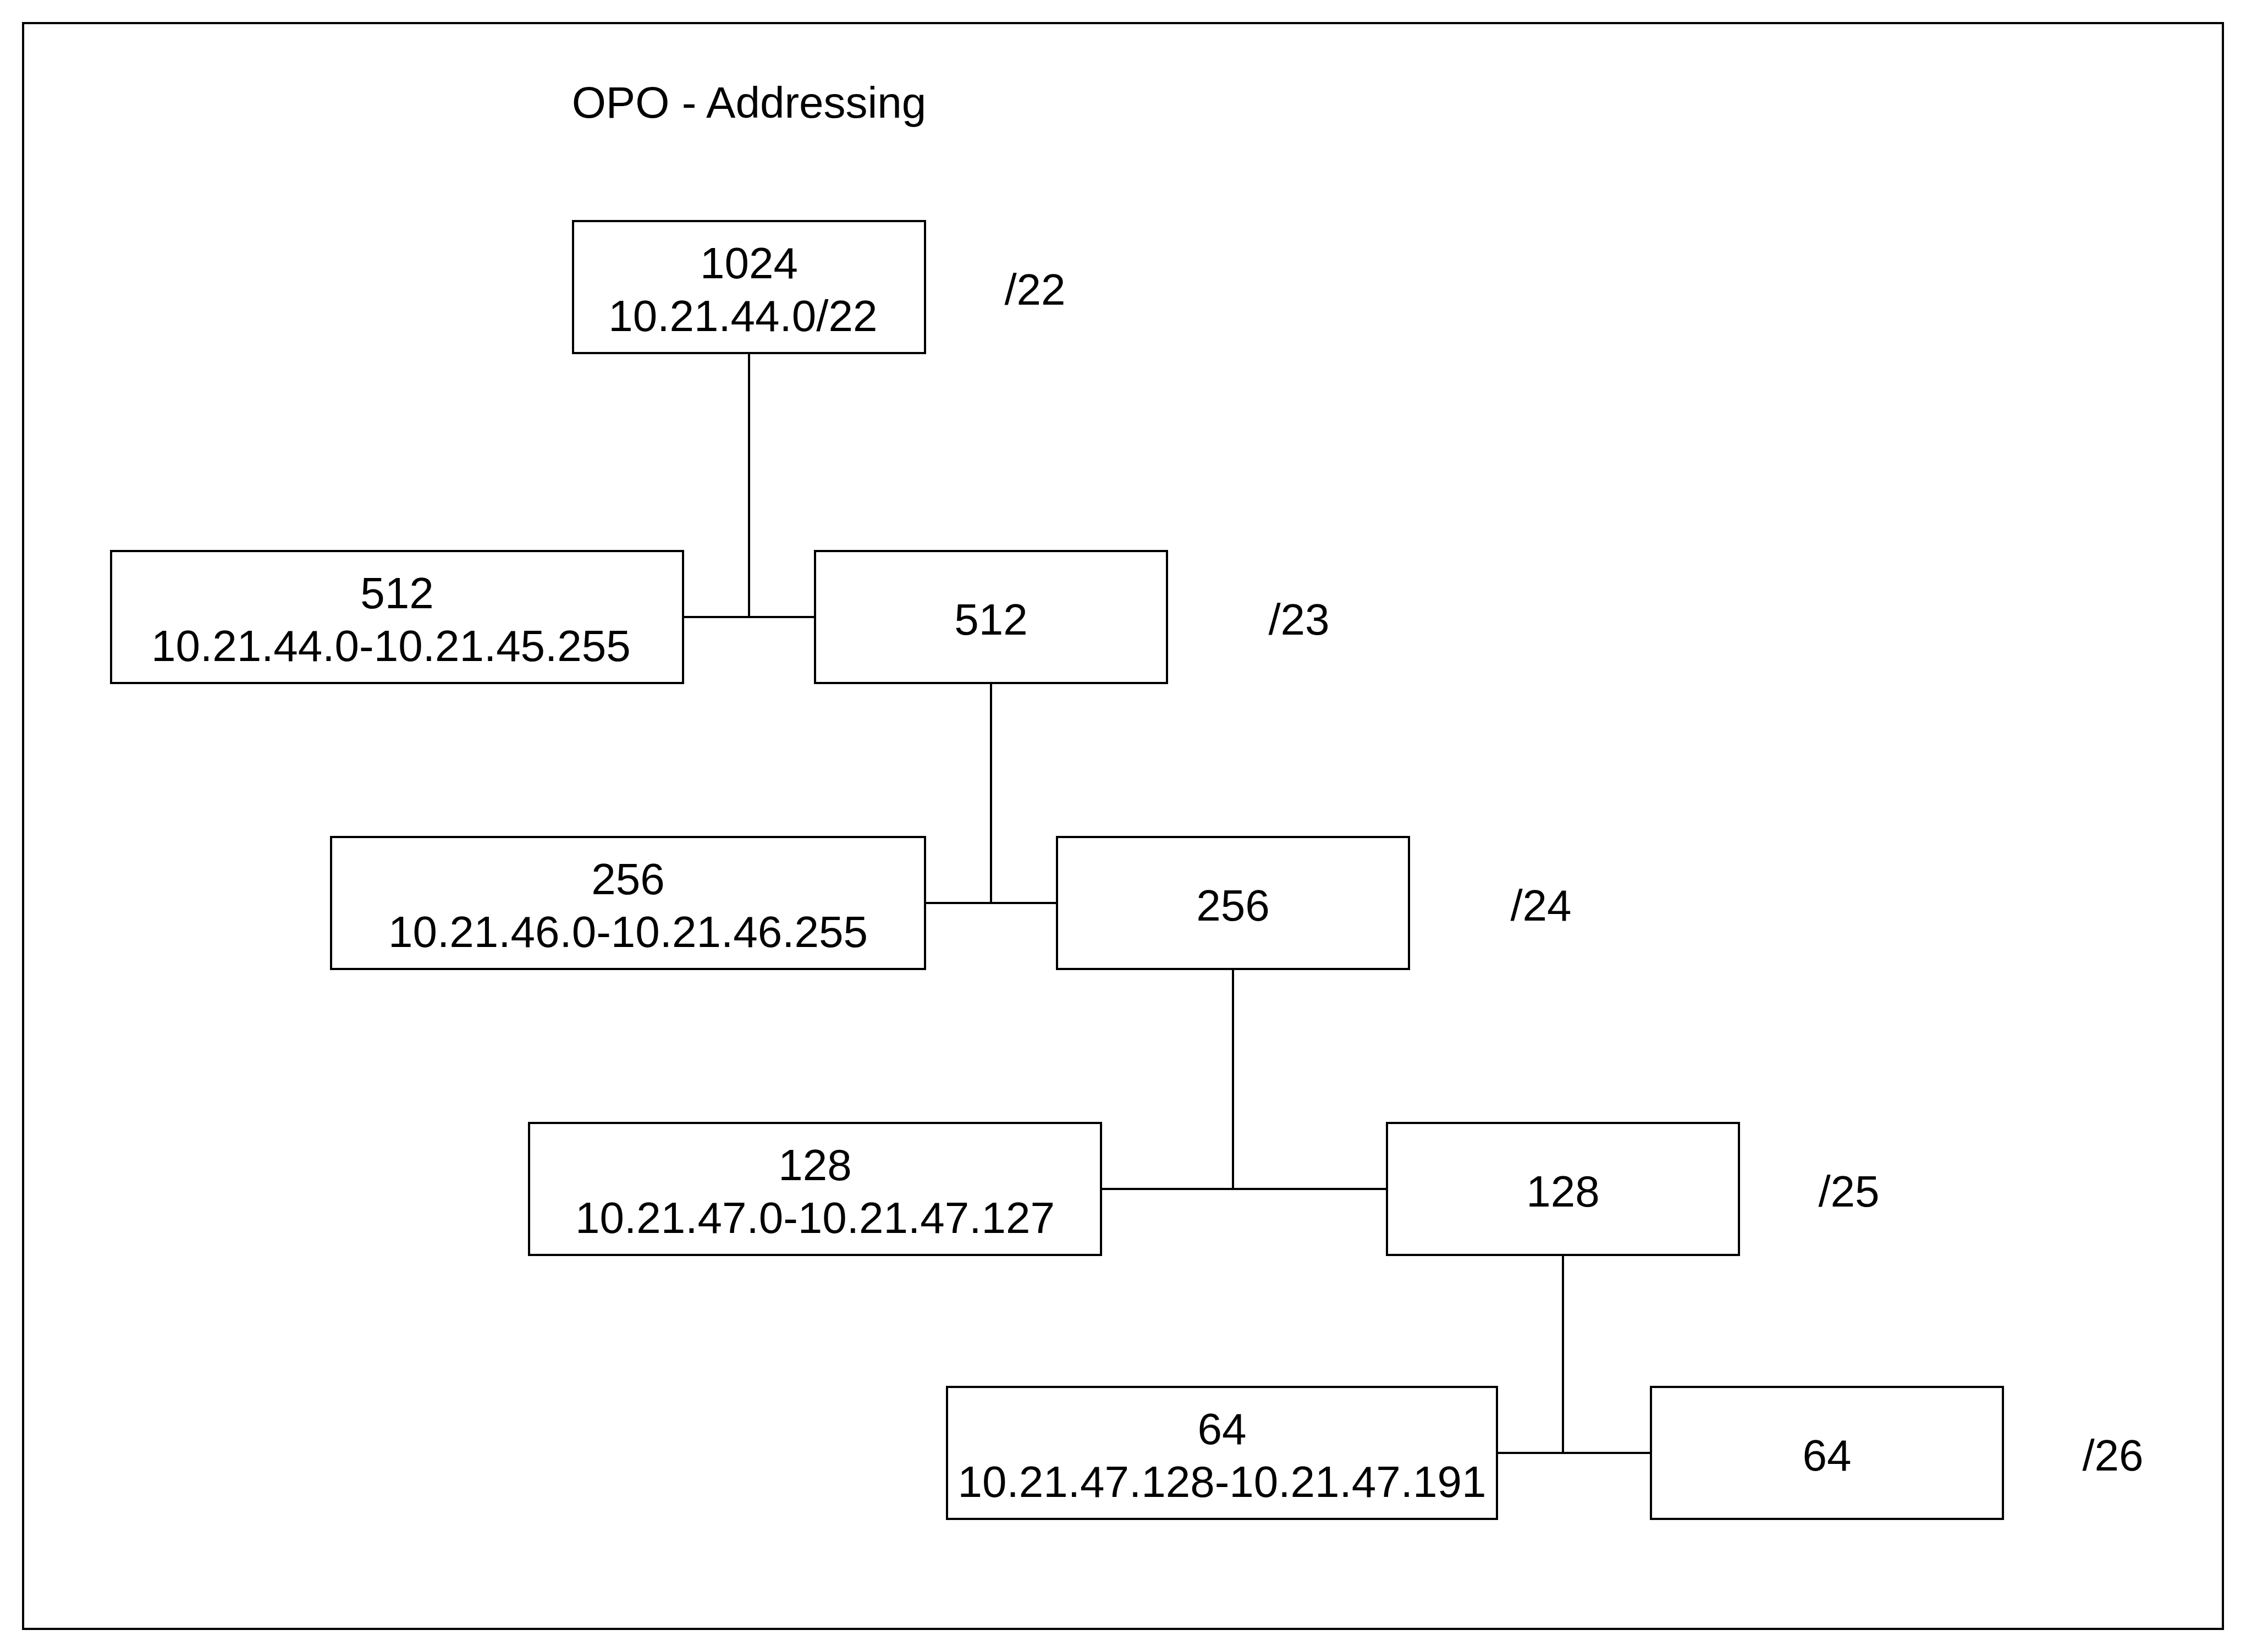
\includegraphics[width=0.8\textwidth]{figures/opo-addressing.png}
\caption{Oporto \ac{WAN} Addressing Diagram\cite{t3a_ipv4_subneting_dhcp}}
\label{fig:opo-addressing}
\end{figure}

This addressing plan ensures that each network has sufficient \ac{IP} addresses to accommodate all devices, while also allowing room for potential future expansion. The subnet sizes were calculated based on the number of hosts in each network, following standard subnetting rules.

\subsection{Equipment Addressing}

The \ac{IP} addresses listed in Table~\ref{tab:ip-plan} correspond to statically assigned management and gateway interfaces within the Oporto headquarters network. These addresses are \textbf{excluded from \ac{DHCP}} to prevent dynamic clients from receiving them.

\medskip

Each VLAN has three reserved addresses:
\begin{itemize}
    \item The \textbf{\ac{HSRP} virtual gateway}, used by hosts as their default gateway.
    \item The \textbf{\ac{SVI} address on MLS1}.
    \item The \textbf{\ac{SVI} address on MLS2}.
\end{itemize}

\noindent
These static \ac{IP}s ensure stable Layer~3 routing and redundancy between MLS1 and MLS2. All other addresses within the \ac{VLAN} subnet ranges are assigned dynamically by the \ac{DHCP} server.


\begin{table}[h!]
\centering
\caption{Network Equipment and Assigned IP Addresses Oporto WAN}
\resizebox{\textwidth}{!}{%
\begin{tabular}{l l l l}
\hline
\textbf{Device} & \textbf{Interface / VLAN} & \textbf{IP Address} & \textbf{Description / Function} \\
\hline
\textbf{HQ Router (2911)} & G0/0 & 10.21.47.193 /30 & Link to MLS1 \\
                          & G0/1 & 10.21.47.197 /30 & Link to MLS2 \\
                          & G0/0/0 & DHCP (Public) & WAN connection to ISP \\[4pt]
\textbf{MLS1 (3560-24PS)} & VLAN10 & 10.21.47.130 /26 & STAFF SVI (HSRP Active) \\
                          & VLAN20 & 10.21.46.2 /24 & ACCOUNTING SVI (HSRP Active) \\
                          & VLAN30 & 10.21.47.2 /25 & HR SVI (HSRP Standby) \\
                          & VLAN40 & 10.21.44.2 /23 & USERS SVI (HSRP Standby) \\
                          & G0/1 & 10.21.47.194 /30 & Link to HQ Router \\[4pt]
\textbf{MLS2 (3560-24PS)} & VLAN10 & 10.21.47.131 /26 & STAFF SVI (HSRP Standby) \\
                          & VLAN20 & 10.21.46.3 /24 & ACCOUNTING SVI (HSRP Standby) \\
                          & VLAN30 & 10.21.47.3 /25 & HR SVI (HSRP Active) \\
                          & VLAN40 & 10.21.44.3 /23 & USERS SVI (HSRP Active) \\
                          & G0/1 & 10.21.47.198 /30 & Link to HQ Router \\[4pt]
\textbf{HSRP Virtual IPs} & VLAN10 & 10.21.47.129 /26 & STAFF Gateway (Virtual) \\
                          & VLAN20 & 10.21.46.1 /24 & ACCOUNTING Gateway (Virtual) \\
                          & VLAN30 & 10.21.47.1 /25 & HR Gateway (Virtual) \\
                          & VLAN40 & 10.21.44.1 /23 & USERS Gateway (Virtual) \\[4pt]
\textbf{SW1, SW2 (2960-24TT)} & Trunk links & N/A & Access layer switches, VTP clients \\[4pt]
\textbf{End Device (PC1)} & VLAN10 & DHCP assigned & STAFF network client \\
\textbf{End Device (PC2)} & VLAN20 & DHCP assigned & ACCOUNTING network client \\
\textbf{End Device (PC3)} & VLAN30 & DHCP assigned & HR network client \\
\textbf{End Device (PC4)} & VLAN40 & DHCP assigned & USERS network client \\
\hline
\end{tabular}%
}
\label{tab:ip-plan}
\end{table}

\section{Configuration}

\subsection{HQ Router and MLS Configuration}
The HQ Router obtains its external \ac{IP} address from the Service Provider via \ac{DHCP}, while the internal connections between the HQ Router and the multilayer switches (MLS1 and MLS2) are configured with static \ac{IP} addresses.  
This ensures consistent routing and stable communication between the HQ and internal networks.

\begin{lstlisting}[caption={HQ Router configuration}, label={lst:hq-router}]
enable
configure terminal

! Internal connection to MLS1
interface GigabitEthernet0/0
 description HQ-MLS1 Connection
 ip address 10.21.47.193 255.255.255.252
 no shutdown
exit

! Internal connection to MLS2
interface GigabitEthernet0/1
 description HQ-MLS2 Connection
 ip address 10.21.47.197 255.255.255.252
 no shutdown
exit

! External connection to Service Provider (WAN)
interface GigabitEthernet0/0/0
 description Service Provider Connection
 ip address dhcp
 no shutdown
exit

! Default route to the Internet (through SP)
ip route 0.0.0.0 0.0.0.0 GigabitEthernet0/0/0
end
\end{lstlisting}

The static \ac{IP}s configured on the HQ Router correspond to the point-to-point subnets used for internal routing with MLS1 and MLS2.

\begin{lstlisting}[caption={MLS1 link to HQ Router}, label={lst:mls1-router-link}]
enable
configure terminal
interface GigabitEthernet0/1
 description Link to HQ Router
 no switchport
 ip address 10.21.47.194 255.255.255.252
 no shutdown
end
\end{lstlisting}

\begin{lstlisting}[caption={MLS2 link to HQ Router}, label={lst:mls2-router-link}]
enable
configure terminal
interface GigabitEthernet0/1
 description Link to HQ Router
 no switchport
 ip address 10.21.47.198 255.255.255.252
 no shutdown
end
\end{lstlisting}

This configuration guarantees reliable Layer~3 communication between the HQ Router and both MLS devices.  
By assigning static \ac{IP} addresses internally and using \ac{DHCP} externally, the HQ Router maintains dynamic Internet access while ensuring stable connectivity with the local switching infrastructure.


\begin{lstlisting}[caption={Access port configuration on SW1 and SW2}, label={lst:sw1-sw2-access}]
interface range fa0/5 - 8
 switchport mode access
 switchport access vlan 10
!
interface range fa0/9 - 12
 switchport mode access
 switchport access vlan 20
!
interface range fa0/13 - 16
 switchport mode access
 switchport access vlan 30
!
interface range fa0/17 - 20
 switchport mode access
 switchport access vlan 40
!
interface range fa0/1 - 4, fa0/21 - 24
 switchport access vlan 99
 shutdown
\end{lstlisting}

\subsection{\ac{VTP} and \ac{VLAN} Configuration}

\ac{VTP} was implemented on the HQ switches in order to automate \ac{VLAN} propagation.  
MLS1 and MLS2 were configured as \ac{VTP} servers and SW1 and SW2 as clients.  
This ensures that \ac{VLAN} information is consistent across all switches.

\begin{lstlisting}[caption={VTP configuration on MLS1 and MLS2}, label={lst:vtp-config}]
vtp domain RECOMP2526TTTGG
vtp password 6252pmocer
vtp mode server
\end{lstlisting}

\begin{lstlisting}[caption={VTP configuration on SW1 and SW2}, label={lst:vtp-clients}]
vtp domain RECOMP2526TTTGG
vtp password 6252pmocer
vtp mode client
\end{lstlisting}

\ac{VLAN}s were created on the MLS switches to segment traffic per department, improving security and broadcast efficiency.

\begin{lstlisting}[caption={VLAN creation on MLS1 and MLS2\cite{tp2_layer2_security}}, label={lst:mls1-msl2-vlans}]
vlan 10 name STAFF
vlan 20 name ACCOUNTING
vlan 30 name HR
vlan 40 name USERS
vlan 50 name NATIVE
vlan 99 name BLACKHOLE
\end{lstlisting}

\subsection{Trunk and Port-Channel Configuration}
To provide redundancy and increased bandwidth between MLS1 and MLS2, a Port-Channel was configured using interfaces \texttt{Fa0/1–2}.  
All inter-switch links were configured as trunks, using \ac{VLAN}~50 as the native \ac{VLAN}.

\begin{lstlisting}[caption={Trunk and Port-Channel configuration on MLS1 and MLS2}, label={lst:mls1-portchannel}]
interface range fa0/1 - 2
 channel-group 1 mode active
!
interface port-channel 1
 switchport trunk encapsulation dot1q
 switchport mode trunk
 switchport trunk allowed vlan all
 switchport trunk native vlan 50
!
interface range fa0/3 - 4
 switchport mode trunk
 switchport trunk allowed vlan all
 switchport trunk native vlan 50
 no shutdown
\end{lstlisting}

This design allows all \ac{VLAN}s to traverse the trunks, ensuring communication between switches and minimizing single points of failure.

\subsection{\ac{RSTP}}
Rapid-PVST was used to optimize convergence and redundancy.  
Root bridge roles were manually assigned to balance \ac{VLAN} traffic: MLS1 for \ac{VLAN}s 10 and 20, and MLS2 for \ac{VLAN}s 30 and 40.

\begin{lstlisting}[caption={RSTP configuration on MLS1}, label={lst:rstp-mls1}]
spanning-tree mode rapid-pvst
spanning-tree vlan 10,20 root primary
spanning-tree vlan 30,40 root secondary
\end{lstlisting}

\begin{lstlisting}[caption={RSTP configuration on MLS2}, label={lst:rstp-mls2}]
spanning-tree mode rapid-pvst
spanning-tree vlan 30,40 root primary
spanning-tree vlan 10,20 root secondary
\end{lstlisting}

This configuration ensures load balancing and prevents loops, as each switch becomes the primary root for specific \ac{VLAN}s.

\subsection{\ac{HSRP} Configuration}
\ac{HSRP} was configured on both MLS switches to provide default gateway redundancy.  
Each \ac{VLAN} has a virtual gateway IP, and the active MLS for each \ac{VLAN} matches its \ac{STP} root, optimizing path efficiency.

\begin{lstlisting}[caption={HSRP configuration on MLS1}, label={lst:hsrp-mls1}]
ip routing
!
interface vlan10
 ip address 10.21.47.130 255.255.255.192
 standby 10 ip 10.21.47.129
 standby 10 priority 110
 standby 10 preempt
!
interface vlan20
 ip address 10.21.46.2 255.255.255.0
 standby 20 ip 10.21.46.1
 standby 20 priority 110
 standby 20 preempt
\end{lstlisting}

\begin{lstlisting}[caption={HSRP configuration on MLS2}, label={lst:hsrp-mls2}]
ip routing
!
interface vlan30
 ip address 10.21.47.3 255.255.255.128
 standby 30 ip 10.21.47.1
 standby 30 priority 110
 standby 30 preempt
!
interface vlan40
 ip address 10.21.44.3 255.255.254.0
 standby 40 ip 10.21.44.1
 standby 40 priority 110
 standby 40 preempt
\end{lstlisting}

This setup guarantees seamless failover for gateway services in the event one switch fails.

\subsection{Layer 2 Switch Configuration}
SW1 and SW2 were configured to connect end devices to the correct \ac{VLAN}s and isolate unused ports.

\begin{lstlisting}[caption={Access port configuration on SW1 and SW2}, label={lst:sw1-access}]
interface range fa0/5 - 8
 switchport mode access
 switchport access vlan 10
!
interface range fa0/9 - 12
 switchport mode access
 switchport access vlan 20
!
interface range fa0/13 - 16
 switchport mode access
 switchport access vlan 30
!
interface range fa0/17 - 20
 switchport mode access
 switchport access vlan 40
!
interface range fa0/1 - 4, fa0/21 - 24
 switchport access vlan 99
 shutdown
\end{lstlisting}

Unused ports were placed in VLAN~99 and shut down to enhance security and prevent unauthorized connections.

\subsection{DHCP Configuration}
Redundant \ac{DHCP} services were configured on both MLS switches.  
Each \ac{VLAN} has its own pool, while addresses used by \ac{HSRP} and \ac{SVI}s were excluded to avoid conflicts.

\begin{lstlisting}[caption={DHCP configuration on MLS1 and MLS2}, label={lst:dhcp-mls}]
ip dhcp excluded-address 10.21.47.129 10.21.47.131
ip dhcp excluded-address 10.21.46.1 10.21.46.3
ip dhcp excluded-address 10.21.47.1 10.21.47.3
ip dhcp excluded-address 10.21.44.1 10.21.44.3
!
ip dhcp pool STAFF
 network 10.21.47.128 255.255.255.192
 default-router 10.21.47.129
 dns-server 8.8.8.8
 domain-name recomp2526.com
\end{lstlisting}

This ensures reliable address distribution and gateway redundancy across all \ac{VLAN}s.


